The \textit{Repository Management} module is responsible for management and cataloging of
algorithms and test data to be used in the benchmarking tests.

\subsection{Domain Model}
The domain model for the Repository Management module is shown in Figure \ref{fig:testDataModel}
\begin{figure}[H]
  \begin{center}
  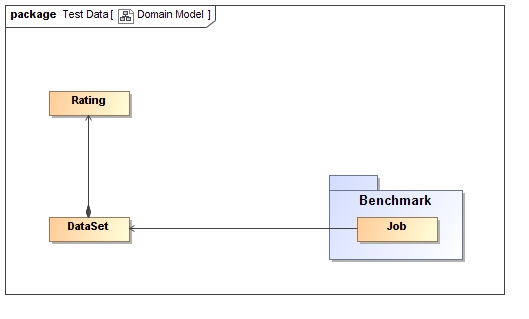
\includegraphics[scale=0.5]{../Diagrams and Charts/Test Data/Domain Model.jpg}  
  \caption{Repository Management Domain Model}
  \end{center}
  \label{fig:testDataModel}
\end{figure}

\subsection{Categories}

\subsubsection{Scope}
The scope for Categories section in Repository Management module is shown in Figure \ref{fig:categoriesRepo}
\begin{figure}[H]
  \begin{center}
  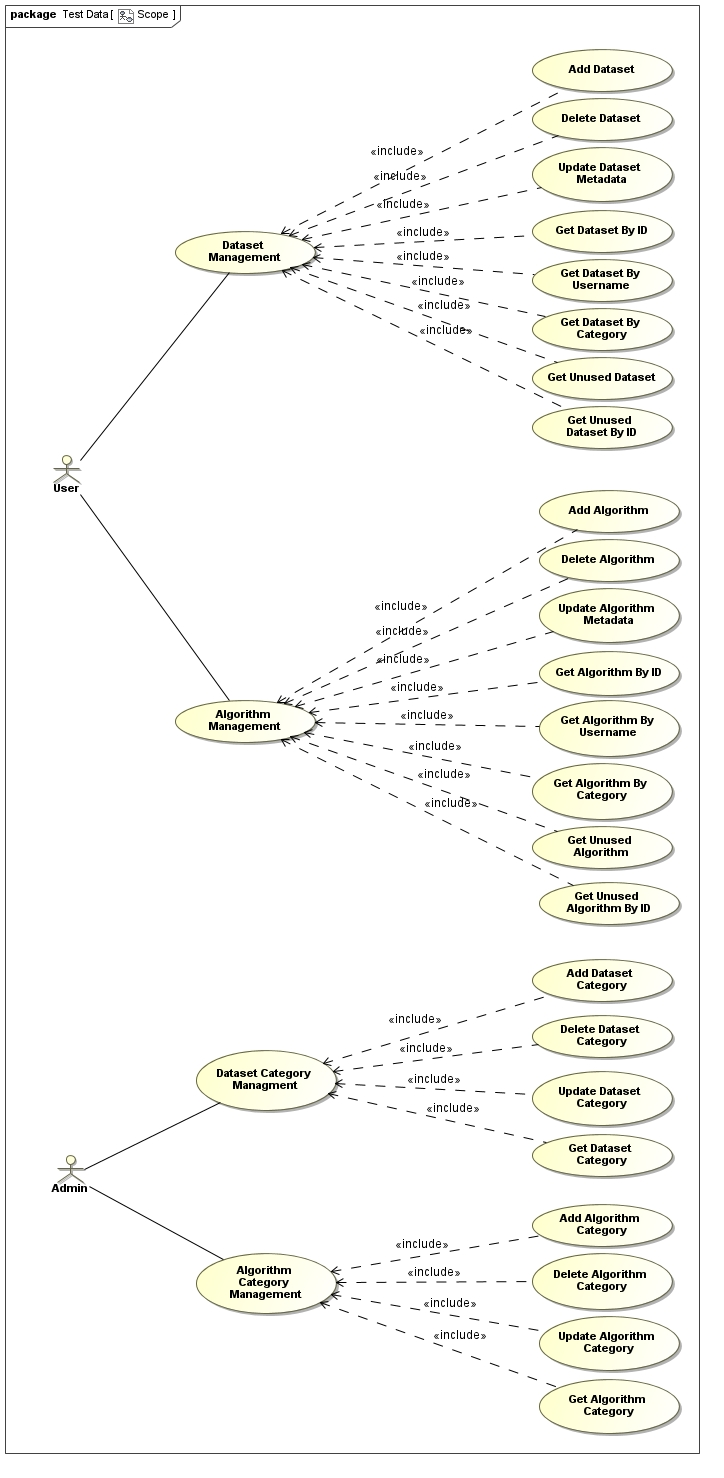
\includegraphics[scale=0.7]{../Diagrams and Charts/Test Data/Scope.jpg}
  \caption{Test Data}
  \end{center}
  \label{fig:categoriesRepo}
\end{figure}
The scope of the Categories section in Repository Management module include:
\begin{itemize}
  \item Admin will be able to create a dataset category.
  \item Admin will be able to delete a dataset category.
  \item Admin will be able to update a dataset category.
  \item Admin will be able to get a dataset category.
\end{itemize}

\subsection{Algorithms}

\subsubsection{Scope}
The scope for Algorithms section in Repository Management module is shown in Figure \ref{fig:algorithmRepo}
\begin{figure}[H]
  \begin{center}
  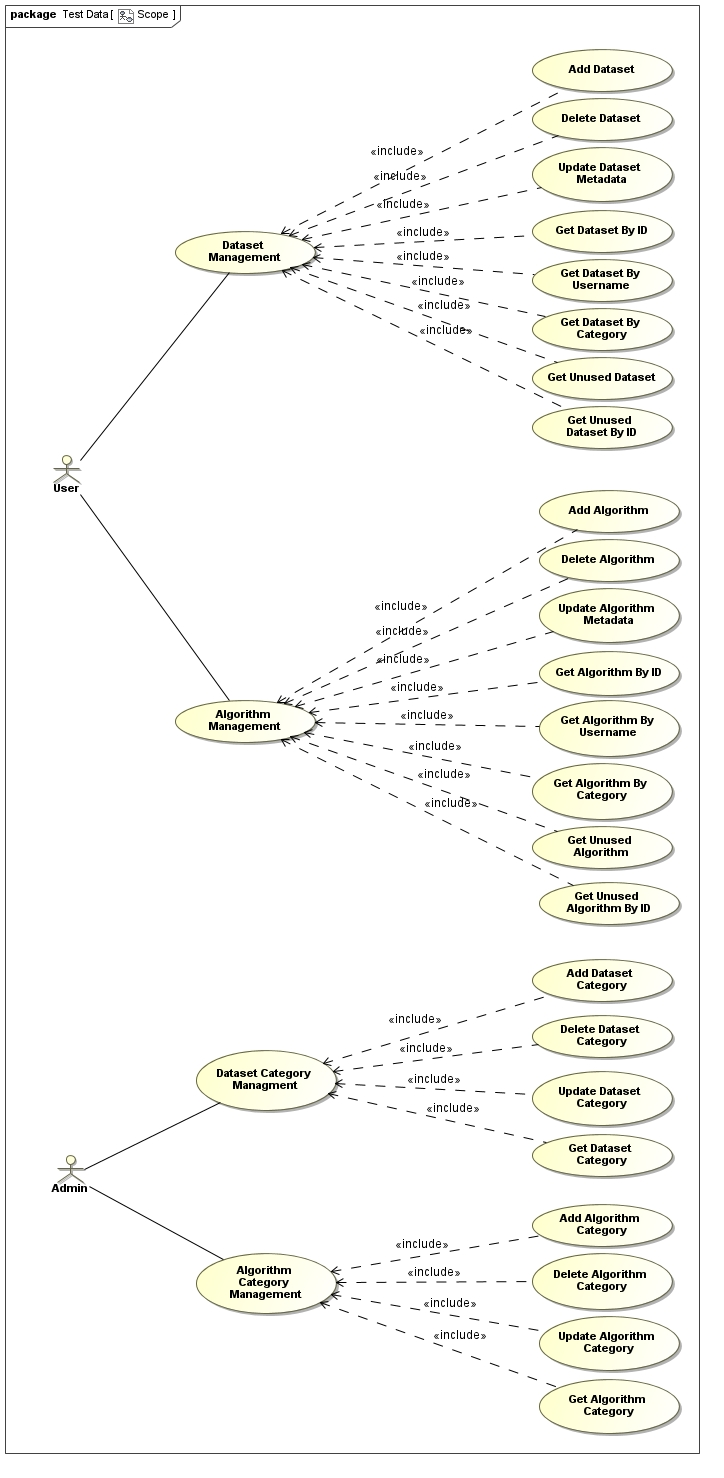
\includegraphics[scale=0.7]{../Diagrams and Charts/Test Data/Scope.jpg}
  \caption{Test Data}
  \end{center}
  \label{fig:algorithmRepo}
\end{figure}
The scope of the Algorithms section in Repository Management module include:
\begin{itemize}

\end{itemize}

\subsection{Dataset}
\subsubsection{Scope}
The scope for Dataset section in Repository Management module is shown in Figure \ref{fig:datasetRepo}
\begin{figure}[H]
  \begin{center}
  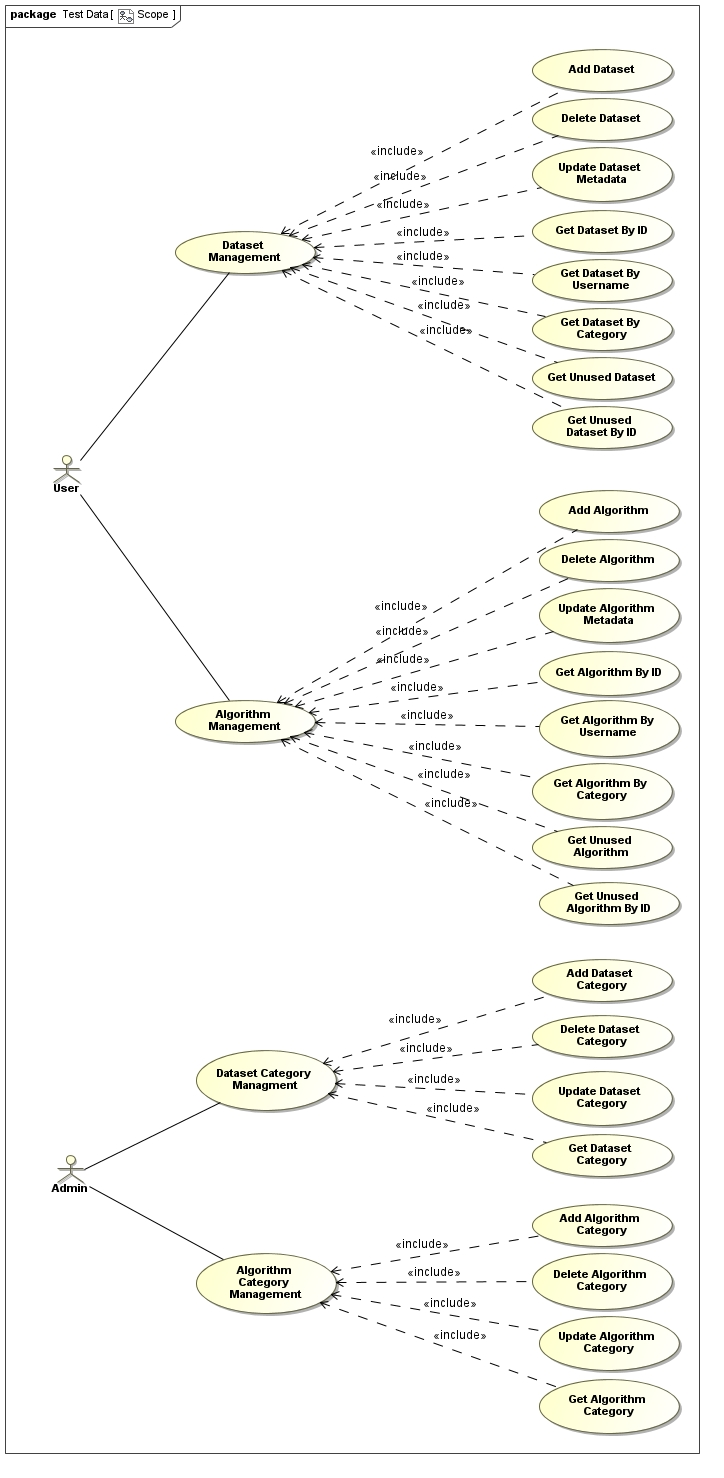
\includegraphics[scale=0.7]{../Diagrams and Charts/Test Data/Scope.jpg}
  \caption{Test Data}
  \end{center}
  \label{fig:datasetRepo}
\end{figure}
The scope of the Dataset section in Repository Management module include:
\begin{itemize}
  \item The user can dynamically generate test data.
  \item Users can rate dynamic or user upload data sets.
  \item Any user can upload there own dataset to the growing repository of data sets.
  \item Users will be able to view the data set with associated meta data.
\end{itemize}





